\overlays{3}{%
  \begin{slide}{Swarm Intelligence}
    Examples of \textit{Swarm Intelligence} found in nature
    \begin{itemize}
      \onlySlide*{1}{%
      \item Flocking birds
	\begin{itemize}
	\item A bird flying disrupts airflow
	\item Disrupted air flow reduces drag for following birds
	\item Reduced drag results in easier flying
	\item Distance traveled by the flock is maximized
	\end{itemize}
	\begin{center}
	  \begin{minipage}{.5\textwidth}
	    \includegraphics[scale=.13]{BirdsFlocking.eps}
	  \end{minipage}
	\end{center}
      }%
      \onlySlide*{2}{%
      \item Foraging ants
	\begin{itemize}
	\item An ant leaves a pheromone trail upon finding food
	\item Other ants follow and reinforce the trail
	\item Each ant is able to find food for the nest
	\item Trail laying finds the closest food source
	\end{itemize}
	\begin{center}
	  \begin{minipage}{.5\textwidth}
	    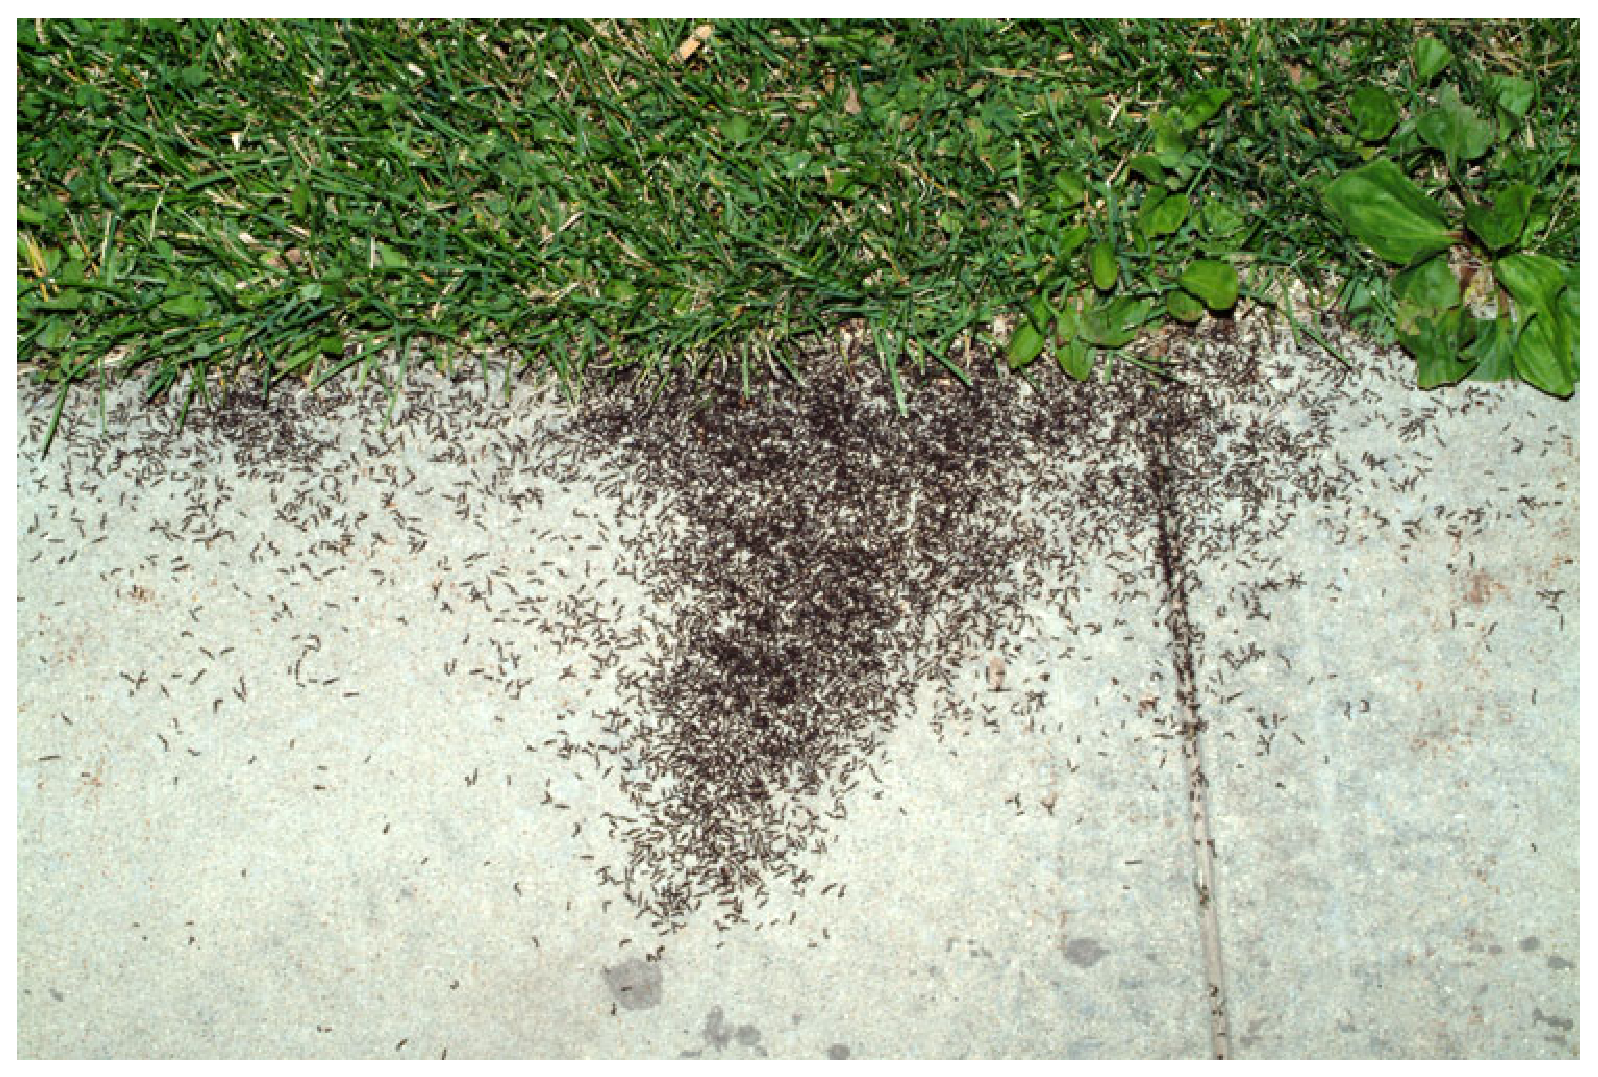
\includegraphics[scale=.2]{AntSwarm.eps}
	  \end{minipage}
	\end{center}
      }%
      \onlySlide*{3}{%
      \item Termite nests
	\begin{itemize}
	\item A termite deposits a pheromone-tagged mud ball
	\item Local pheromones affect mud ball placement
	\item A secure nest for the termite is established
	\item A temperature regulated nest emerges
	\end{itemize}
	\begin{center}
	  \begin{minipage}{.5\textwidth}
	    \centering
	    \includegraphics[scale=.17]{TermiteNest.eps}
	  \end{minipage}
	\end{center}
      }%
    \end{itemize}
  \end{slide}
}%

%%%%%
%%%%%

\begin{slide}{Swarm Intelligence}
  % evolution has produced swrming in many different contexts
  Why has evolution produced swarming in so many different contexts?
  \begin{itemize}
    \itemsep=3ex
    \bigskip
  \item Simultaneously benefits the individual and the whole
  \item Individuals benefit from the efforts of others
    % as a meta-entity or organism
  \item The survivability of the swarm increases
    % its ``easy''...in retrospect
  \item Simple rules and behaviors, decentralized
  \item Replication relatively easy
  \end{itemize}
\end{slide}

%%%%%
%%%%%

\begin{slide}{Swarm Intelligence}
  Swarm intelligence as defined for this work
  
  \begin{quote}
    a group of agents whose collective interactions magnify the
    effects of individual agent behaviors, resulting in the
    manifestation of swarm level behaviors beyond the capability of
    a small subgroup of agents
  \end{quote}
  
  Other properties required for emergent behavior
  \begin{itemize}
  \item Large numbers of agent interactions
    % these create feedback, thus affecting the agent's context
    % continued feedback accumulates, bigger feedback than by any single agent
  \item Ability to modify the environment, stigmergy
  \item Randomness
  \end{itemize}
\end{slide}

